
\documentclass[a4paper,10pt,left=1.5cm,right=1.5cm,top=1.5cm,bottom=1.5cm]{article}

\usepackage{geometry}

\geometry{a4paper,left=4.5cm,right=3cm,top=1cm,bottom=2cm}

\usepackage[utf8x]{inputenc}
\usepackage{url}
\usepackage[ngerman]{babel}
\usepackage{graphicx}

\parindent 0pt 
\parskip 10pt

\title{4. Praktikum: Modellierung von Dynamischen Systemen}
\author{Andreas Krohn \and Benjamin Vetter}

\begin{document}

\maketitle

\tableofcontents

\section{Vorbereitung: Modellierung des Wirkungsdiagramms}

\subsection{Bestimmen Sie für den Arbeitspunkt (x0=15mm) den Strom i0 und die Spannung u0}

Es gilt:

\begin{equation}
  m\ddot{x}=\sum F=mg-C(\frac{i}{x})^2
\end{equation}

Für den Strom $i_0$ gilt:

\begin{eqnarray*}
  0 = mg-C(\frac{i}{x})^2 \\
  C(\frac{i}{x})^2 = mg \\
  (\frac{i}{x})^2 = \frac{mg}{C} \\
  \frac{i}{x} = \sqrt{\frac{mg}{C}} \\
  i = x\sqrt{\frac{mg}{C}} \\
  i = 0.015m \sqrt{\frac{0.025kg \cdot 9.81 \frac{m}{s^2}}{5 \cdot 10^{-6} \frac{\frac{kg \cdot m}{s^2} m^2}{A^2}}} \\
  i = 0.015m \sqrt{0.025kg \cdot 9.81 \frac{m}{s^2} \cdot \frac{1}{5 \cdot 10^{-6}} \frac{A^2}{\frac{kg \cdot m^3}{s^2}}} \\
  i = 0.015m \sqrt{0.025kg \cdot 9.81 \frac{m}{s^2} \cdot \frac{1}{5 \cdot 10^{-6}} \cdot A^2 \cdot \frac{s^2}{kg \cdot m^3}} \\
  i = 0.015m \sqrt{\frac{0.025 \cdot 9.81}{5 \cdot 10^{-6}} \cdot \frac{A^2}{m^2}} \\
  i = 3.3221 A
\end{eqnarray*}

Für die Spannung $u_0$ gilt:

\begin{equation}
  u(t) = R \cdot i(t) + L \cdot \frac{di(t)}{dt}
\end{equation}

Es gilt:

\begin{eqnarray*}
  u_0 = 3 \frac{V}{A} \cdot 3.3221 A + 0.1 \frac{Vs}{A} \cdot \frac{di(t)}{dt} \\
  u_0 = 3 \frac{V}{A} \cdot 3.3221 A + 0 \\
  u_0 = 9.9663 V
\end{eqnarray*}

\subsection{Zeichnen Sie für die DGLn (1) und (2) die Strukturbilder (Integrierer, Funktionen, ...)}

\begin{eqnarray*}
  \ddot{x} = g - \frac{C}{m} \cdot (\frac{i}{x})^2
\end{eqnarray*}

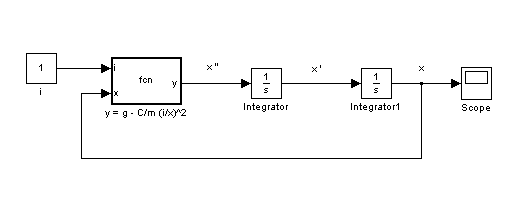
\includegraphics[width=1\textwidth]{dgl1.png}
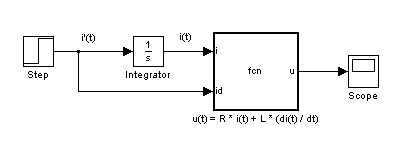
\includegraphics[width=0.8\textwidth]{dgl2.png}

\subsection{Linearisieren Sie die DGLn (1) und (2)}

Es gilt:

\begin{eqnarray*}
  \ddot{x} = g - \frac{C}{m} \cdot (\frac{i}{x})^2 \\
  \ddot{x}(t) = g - \frac{C}{m} \cdot (\frac{i(t)}{x(t)})^2 \\
\end{eqnarray*}

Nach $di$ im AP abgelitten:

\begin{eqnarray*}
  \frac{\delta f}{\delta i} \bigg\vert_A = - \frac{2 C i_0}{mx^2} \\
& = - 2 \cdot 5 \cdot 10^{-6} \frac{kg \cdot m^3}{A^2 s^2} \cdot 3.3221 A \cdot \frac{1}{0.025 kg \cdot 0.015^2 m^2} \\
& = - \frac{2 \cdot 5 \cdot 10^{-6} \cdot 3.3221}{0.025 \cdot 0.015^2} \frac{m}{A s^2}\\
& = -5.9060 \frac{m}{A \cdot s^2}
\end{eqnarray*}

Nach $dx$ im AP abgelitten:

\begin{eqnarray*}
 \frac{\delta f}{\delta x} \bigg\vert_A = \frac{2 C i_0^2}{m x^3} \\
& = 2 \cdot 5 \cdot 10^{-6} \frac{kg \cdot m^3}{A^2 s^2} 3.3221^2 A^2 \cdot \frac{1}{0.025 kg \cdot 0.015^3 m^3} \\
& = \frac{2 \cdot 5 \cdot 10^{-6} \cdot 3.3221^2}{0.025 \cdot 0.015^3} \frac{1}{s^2} \\
& = 1308.0120 \frac{1}{s^2}
\end{eqnarray*}

Daraus folgt:

\begin{equation}
  \Delta \ddot{x} = - 5.9060 \frac{m}{A s^2} \cdot \Delta i + 1308.0120 \frac{1}{s^2} \cdot \Delta x
\end{equation}

Es gilt:

\begin{eqnarray*}
  u(t) = R \cdot i(t) + L \cdot \dot{i}(t) \\
  \dot{i}(t) = \frac{1}{L} \cdot u(t) - \frac{R}{L} \cdot i(t)
\end{eqnarray*}

Nach $di$ im AP abgelitten:

\begin{eqnarray*}
  \frac{\delta f}{\delta i} \bigg\vert_A = - \frac{R}{L} \\
& = - 3 \frac{V}{A} \cdot 10 \frac{A}{Vs} \\
& = - 30 \frac{1}{s}
\end{eqnarray*}

Nach $du$ im AP abgelitten:

\begin{eqnarray*}
  \frac{\delta f}{\delta u} \bigg\vert_A = \frac{1}{L} \\
& = \frac{1}{0.01 \frac{Vs}{A}} \\
& = 10 \frac{A}{Vs}
\end{eqnarray*}

Daraus folgt:

\begin{equation}
  \Delta \dot{i} = -30 \frac{1}{s} \cdot \Delta i + 10 \frac{A}{Vs} \cdot \Delta u
\end{equation}

\subsection{Normieren Sie die linearisierten DGLn auf SI-Größen}

(3) liegt bereits in SI-Einheiten vor.

Für (4) gilt:

\begin{eqnarray}
  \Delta \dot{i} = -30 \frac{1}{s} \cdot \Delta i + 10 \frac{s^2 A^2}{m^2 kg} \cdot \Delta u
\end{eqnarray}

TODO?

\subsection{Geben Sie zu den linearisierten und normierten DGLn die Übertragungsfunktionen an}

\begin{eqnarray*}
  s^2 X(s) - 1308.012 s^0 X(s) = -5.9060 s^0 I(s) \\
  X(s)(s^2 - 1308.012) = -5.9060 I(s) \\
  G_1(s) = \frac{X(s)}{I(s)} = \frac{-5.9060}{s^2 - 1308.012}
\end{eqnarray*}

\begin{eqnarray*}
  s^1 I(s) + 30 s^0 I(s) = 10 s^0 U(S) \\
  I(s)(s + 30) = 10 U(s) \\
  G_2(s) = \frac{I(s)}{U(s)} = \frac{10}{s + 30} 
\end{eqnarray*}

\subsection{Geben Sie die Gesamtübertragungsfunktion der Regelstrecke an}

\begin{equation}
  G(s) = G_1(s) \cdot G_2(s) = - \frac{59.060}{s^3 + 30 s^2 - 1308.0120 s - 39240.36}
\end{equation}

\end{document}

